\section{Arbeitspaket 3.3}

\subsection{Access Monitoring}

\begin{frame}{Access Monitoring through Applications}
    \begin{itemize}
        \item Monitoring von Datenzugriffen
        \item Wie oft kann eine I/O Anfrage lokal bearbeitet werden?
        \item Wie oft muss f\"{u}r eine I/O Anfrage kommuniziert werden?\\
            Wieviel zus\"{a}tzliche Zeit wird daf\"{u}r ben\"{o}tigt?
        \item Welche Dateien oder Dateisystembl\"{o}cke, werden
            von welchen Prozessen oder Knoten zugegriffen?
    \end{itemize}
    \begin{block}{Ziel}
        Diese Informationen stellen den Input f\"{u}r das "Data-Placement" da.
        Die Ergebnisse werden "pro Anwendungs-Lauf" gespeichert.
        Das Format soll einfach aggregierbar sein und in einer Datenbank gespeichert
        werden.
    \end{block}
\end{frame}


\begin{frame}{eBPF - extended Berkley Packet Filter}
    \begin{itemize}
        \item virtuelle Maschine innerhalb des Kernels
        \item BPF Programm wird aus dem User-Space geladen.
        \item Just-in-Time Compiler konvertiert BPF Code in nativen Bytecode.
        \item Ausf\"{u}hrung h\"{a}ngt an einem KProbe oder UProbe.
        \item abgefragte Daten werden in den User-Space kopiert
        \item ben\"{o}tigt aktuellen Kernel
    \end{itemize}
\end{frame}

\begin{frame}{eBPF - extended Berkley Packet Filter}
    \begin{figure}
        \centering
        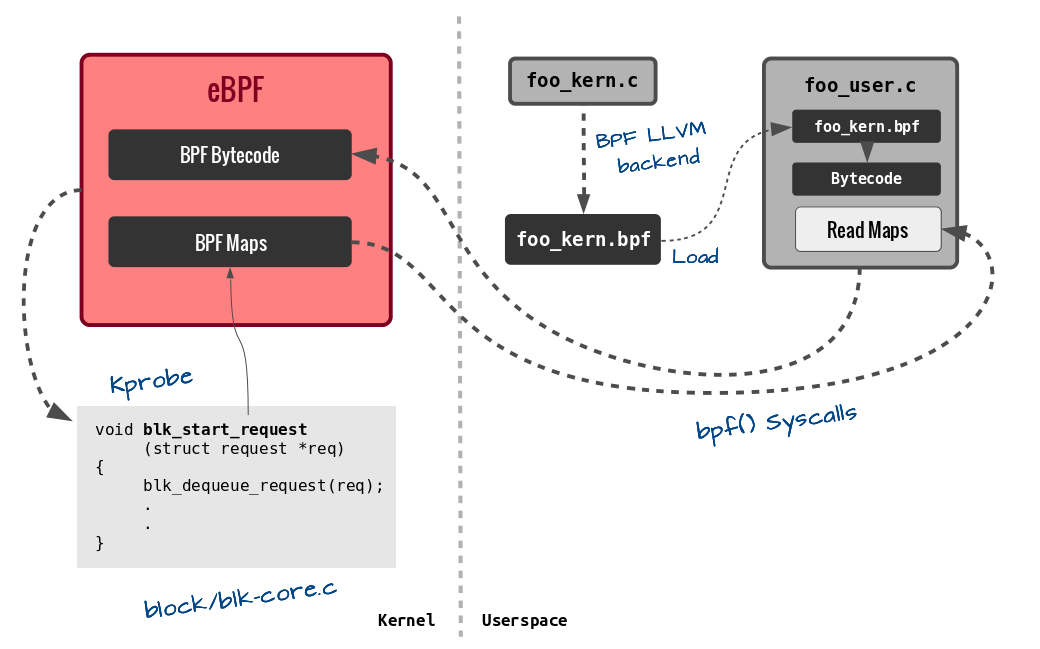
\includegraphics[width=0.98\textwidth]{fig/ebpf-session.png}
    \end{figure}
    \tiny{\href{eBPF}{https://suchakra.files.wordpress.com/2015/08/ebpf-session.png}}
\end{frame}

\begin{frame}{Workflow: Monitoring}
    \begin{enumerate}
        \item Eintrag pro Anwendungslauf.
        \item Abfragen der Informationen \"{u}ber Monitoring-Schnittstellen.
        \item Speichern in der Datenbank.
        \item Aggregationen in der Datenbank.
    \end{enumerate}
\end{frame}

\subsection{Monitoring Visualization}

\begin{frame}{Auswertung}
    \begin{itemize}
        \item Tools zur Datenbankabfrage der Monitoring Daten.
        \item Support f\"{u}r verschiedene Ausgabeformate.
        \item Visualisierung der Daten.
    \end{itemize}
\end{frame}
